\documentclass[english]{tktltiki}
\usepackage[pdftex]{graphicx}
\usepackage{subfigure}
\usepackage{booktabs}
\usepackage{url}
\usepackage{amsthm,amssymb}
 \usepackage{amsmath}
\begin{document}
\onehalfspacing

\title{Observation of an office of an IT firm}
\author{P�ter Ivanics}
\date{\today}

\maketitle

\numberofpagesinformation{\numberofpages\ pages + \numberofappendixpages\ appendices}

\section{Introduction}
This short report summarizes the findings of the "Observation" assignment given on the Designing Interactive Systems course. The goal of the observation is to learn about and discover a daily experience of employees working at a software company. By software company we mean businesses, whose main purpose and aim is software development, the monetizing and selling of their solution and/or software product(s).

The main aim of the observation is to discover is the regular habits, values and challenges of the stakeholders presented on Figure \ref{stakeholder_map} in such environment. These may include internal practices at the firm, tangible or intangible means, software or hardware components, relationships or habits of individuals. 

Typically different companies have slightly different company culture. Nevertheless, the challenges, problems and some tasks faced by individual companies share similarities. For example, overcoming the challenges created by in intercultural environment, employee well-being and satisfaction, leadership, short and long term planning, time-scheduling or work-free time balance of employees are widely faced challenges along different fields. The motivation behind selecting such environment is the possibility to generalize the findings widely and project them onto a similar, but essentially different environment. Nowadays there is a high number of companies operating in software-related areas.

For convenience, the current workplace of the researcher is selected as a case company. The company is a Helsinki-based firm of around 10 employees who deliver solutions in mobile workforce management internationally to various business verticals. For privacy reasons, the name of the company and its employees are kept anonymous. Please note that as the sample is limited to a single company and observation and therefore the results of this report are not sufficient to generalize them onto a wide scope. To do so, further observations and other type of data collection methods, such as interviews, in various setting should be conducted and analyzed.  

\section{Stakeholder map}
The stakeholder map of the analyzed office environment is listed below (Figure \ref{stakeholder_map}). The main stakeholders to focus on are employees, employers, customers and cleaners who visit the office on a regular basis. Despite the fact that other stakeholders are displayed on the map, they are excluded from the analysis due to its reduced scope. 

	\begin{figure}[h] 
		\begin{center}
			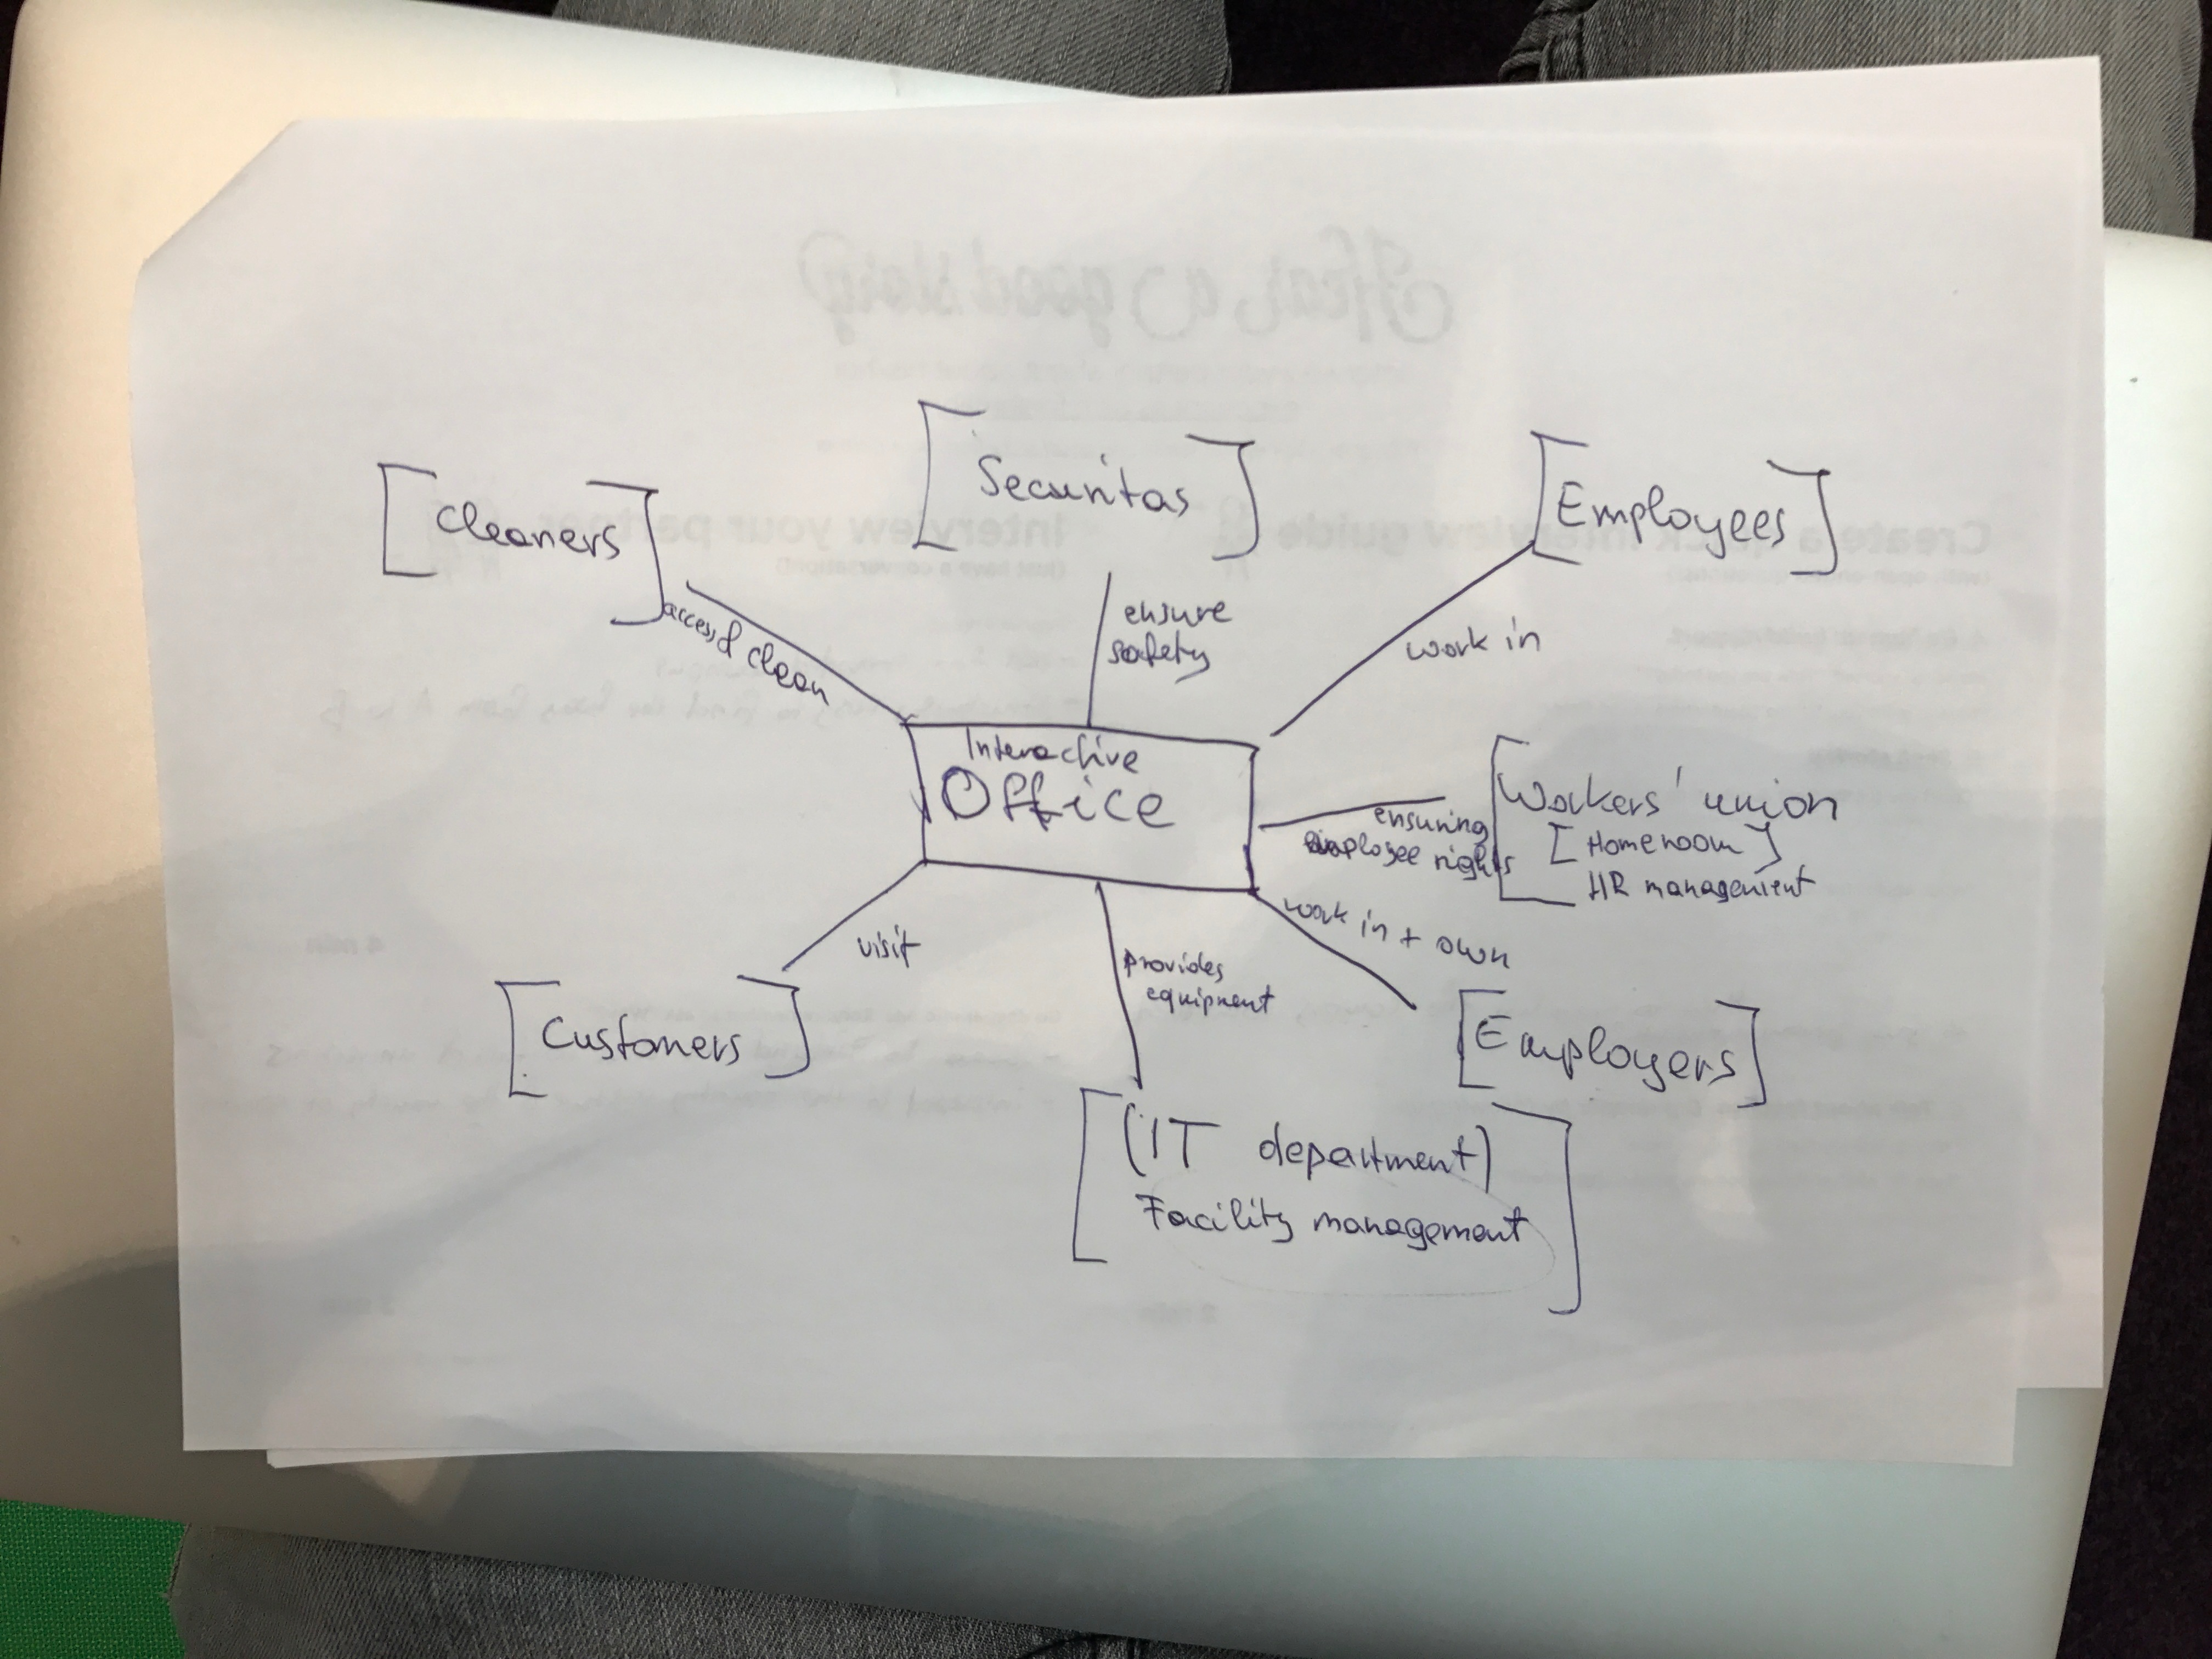
\includegraphics[width=0.9\textwidth]{images/stakeholdermap.jpg}
			\caption{The stakeholder map in an office environment.}
			\label{stakeholder_map}
		\end{center}
	\end{figure}
	
To give more understanding to the context, let us take a look at the the relationships among these stakeholders. Essentially, the above listed stakeholders visit their working environment on a regular basis to perform their job. Depending on the situation and role filled in by individuals at the firm, the regularity of visiting the office environment may differ. Nevertheless, the purpose remains the same and the "effectiveness" of the work is clearly a key aspect for all stakeholders. If one visits their work environment, their aim is to get their job done effectively. 

Effectiveness of work may depend on multiple dimensions such as how creative the work environment is, which practices employees use to cooperate, how well those practices fit their team spirit, does the environment facilitate creativity and last but not least, what is the mental state and level of well being of the involved parties. 

In this respect, there is a clear relationship between employers (supervisors) and employees which requires the establishment of an environment, that can get the best possible outcome of the team working in the office. This involves role delegation, company culture, strategy and employee satisfaction. On top of that, employers typically have the role to motivate their employers to enhance their commitment and motivation towards work. Similarly, employees may aim work an intellectually stimulating workplace by challenging themselves with professionally demanding tasks and by learning from respective colleagues. 

At the same time, employers aim to maximize business value and revenue. For this reason, it is essential to have a highly committed and motivated team behind the company strategy. Every now and then, the customers of the firm visit the office on-site and seek the trust and confidence in their business partner. Companies having such workforce unconsciously give a good impression towards the customer as the trust is established by seeing individuals' commitment and joy at their work. 

Last, but not least, cleaners play a role to maintain the hygiene of the working environment. Their aim and goals towards the office environment is different and typically do not interact too much with the employees nor the management of the company who owns the facilities. However, they visit with very similar task-list and perform similar actions on a regular (in some cases even daily) basis in multiple, similar offices. Despite the fact that there is not too many relationship between them and other stakeholders, they would benefit from solutions supporting their repetitive tasks and assist them to perform those quicker. 

\section{Observation and insights}
The observation is carried out on a regular workday in the office when most of the employees are present. The room in which the observation is done is shared with four other colleagues and is a "connective" room between a corridor and a room in which other people are working. Therefore, there are multiple people actively working in the room and occasionally others pass through the room. Accordingly, the room is fairly noisy in general and there is some movement between employees. The room is equipped with rising desks and a whiteboard, that is used for work often by the employees. 

I went to the office early enough to set up my devices and prepare myself for the observation. My colleagues were not informed about the research in progress as I wanted to observe the environment in its natural setting. The observed insights and their short descriptions are, as follows:

\begin{enumerate}
	\item \textbf{Arrival to the office}: the first employees started to come around 9 AM and began to work in piece. As more and more people arrived to the office, the level of noise, interaction and movement increased naturally. Typically newcomers greeted their colleagues and initiated casual conversations with fellow coworkers (e.g. by asking how are you today, how was last afternoon, did you get stuck in the traffic as well?). However, some workers just entered the room with a coffee, sat down and began to work. 
	\item \textbf{Meetings}: around 10 AM, some colleagues left for a regular Daily Scrum meeting, which was hosted in another room. Throughout the working days, there are many prescheduled and recurring meetings, which are always hosted in one of the meeting rooms. Others left to their own private meetings/Skype calls during the day so that others are not disturbed and remain focused. In some cases however, people had ad-hoc face-to-face meetings or phone calls in the room which increased the level of noise and disturbance towards others.
	\item \textbf{Noise and interruption}: noise tended to be disturbing in some situations to employees. In most cases once somebody entered the room, he or she began to talk to one of their colleagues which dragged the attention of other workers in the zone. The disturbed employees either joined the conversation (which was either casual or work-related) and changed their attention from their computers to the person who just entered the room. This may or may not be a problem as these interruptions can be constructive to employee relationships or knowledge sharing in the company, but some may consider them as unnecessary interruptions. 	
	\item \textbf{Light in the room}: one interesting observation made during the day was pointed out by one of the employees in the office. Namely, the room has only one window and there is no natural light source coming in from the street. This fact is annoying for employees who work in this room for a long time as days are very short during the Finnish winter and there is not too much natural light whatsoever. For this reason, the company installed a device (similar to the one displayed on Figure \ref{artificial_sunlight}) that provides artificial sunlight that is turned on most of the day. 
	
	\begin{figure}[h] 
		\begin{center}
			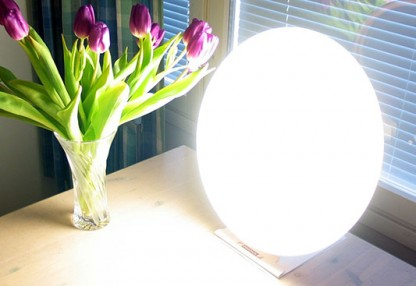
\includegraphics[width=0.9\textwidth]{images/artificial_sunlight.jpg}
			\caption{The office is equipped with a device that provides artificial light to the room with weak access to natural sunlight (the picture is only an illustration).}
			\label{artificial_sunlight}
		\end{center}
	\end{figure}
	\item \textbf{Interaction and breaks}: despite the morning chit-chat and the meetings, colleagues did not interact too much. Mostly, people were into their computers and their work, some even so much that seemingly they did not take any break despite lunch. 
	\pagebreak
	\item \textbf{Cleaning service}: at the end of the day, the cleaners arrived to the office. Their duties during workdays seemed to be limited to gather all glasses and cutlery from the desks of the employees and bring them to the common kitchen on the floor. Seemingly, the only cleaning lady had to make several rounds between the kitchen and the different rooms as the employees left many dishes all around the office. This seemed to be time consuming and probably would have been much faster if the items would be in the kitchen already. 
\end{enumerate}

\lastpage

\pagestyle{empty}
\end{document}